\section{Resultados}

\begin{frame}[plain]
    \begin{tikzpicture}[remember picture,overlay]
        \node[align=center, text=black, font=\huge\bfseries, text width=13cm]
            at (current page.center)
            {¿La variabilidad entre sujetos\\[2mm]
            oculta la separación emocional?};
    \end{tikzpicture}
\end{frame}

\begin{frame}{Separabilidad global: PCA}
    \begin{columns}[T,onlytextwidth]
        \begin{column}{0.49\textwidth}
            \centering
            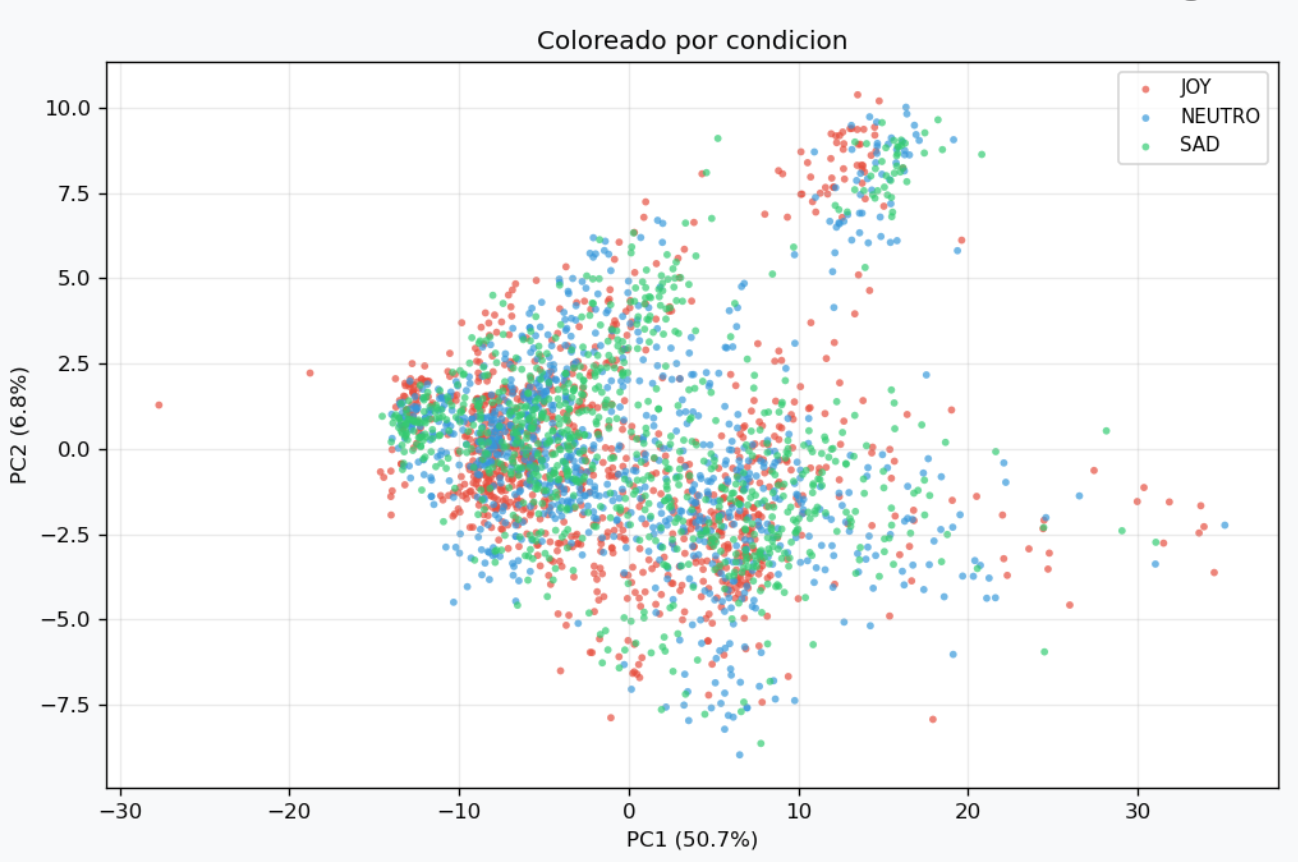
\includegraphics[width=0.94\linewidth]{../memoria/figs/separability/PCA_global_condicion.png}
            \vspace{1mm}

            {\scriptsize Color por condición emocional}
        \end{column}
        \begin{column}{0.49\textwidth}
            \centering
            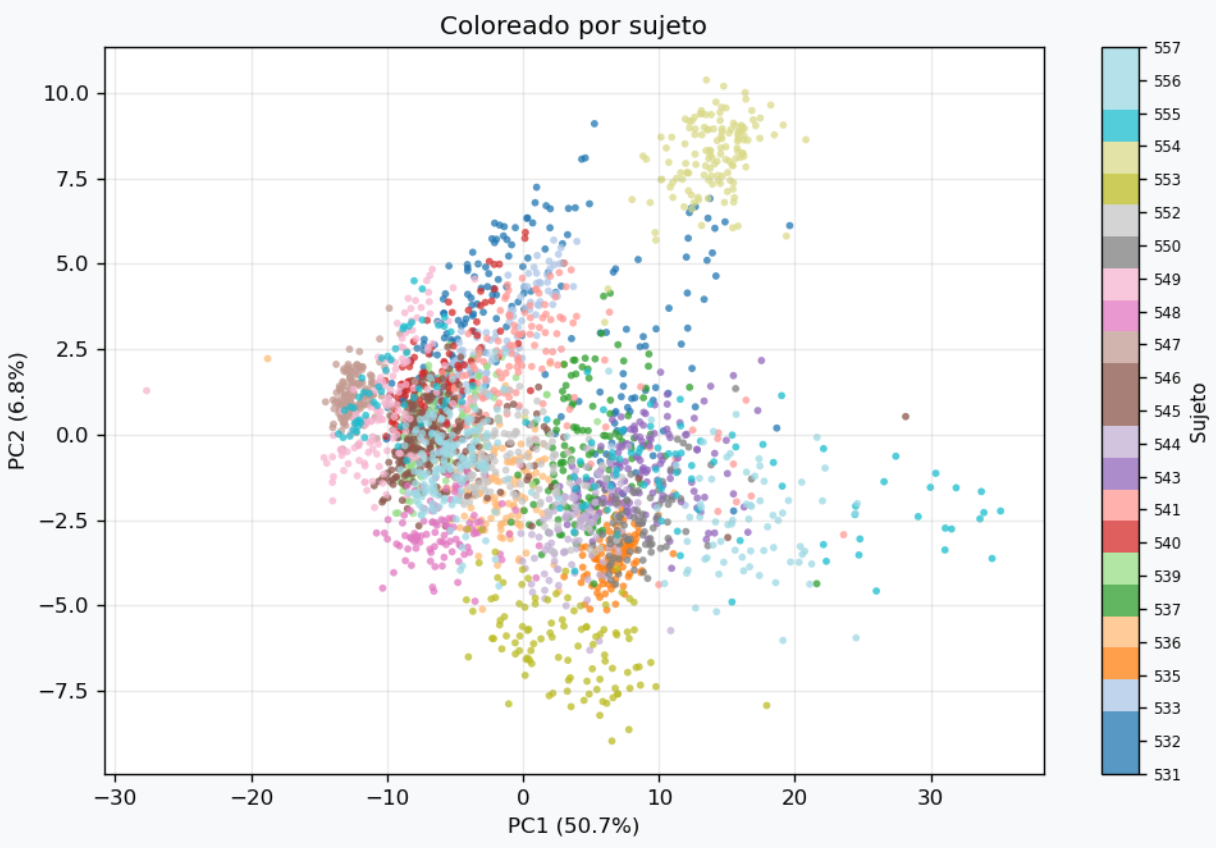
\includegraphics[width=0.94\linewidth]{../memoria/figs/separability/PCA_global_sujeto.png}
            \vspace{1mm}

            {\scriptsize Color por sujeto}
        \end{column}
    \end{columns}

    \vspace{3mm}
    \centering
    {\small La PCA global permite comprobar si la variabilidad principal se organiza mejor por emoción o por diferencias entre participantes.}
\end{frame}

\begin{frame}{Separabilidad global: LDA}
    \begin{columns}[T,onlytextwidth]
        \begin{column}{0.49\textwidth}
            \centering
            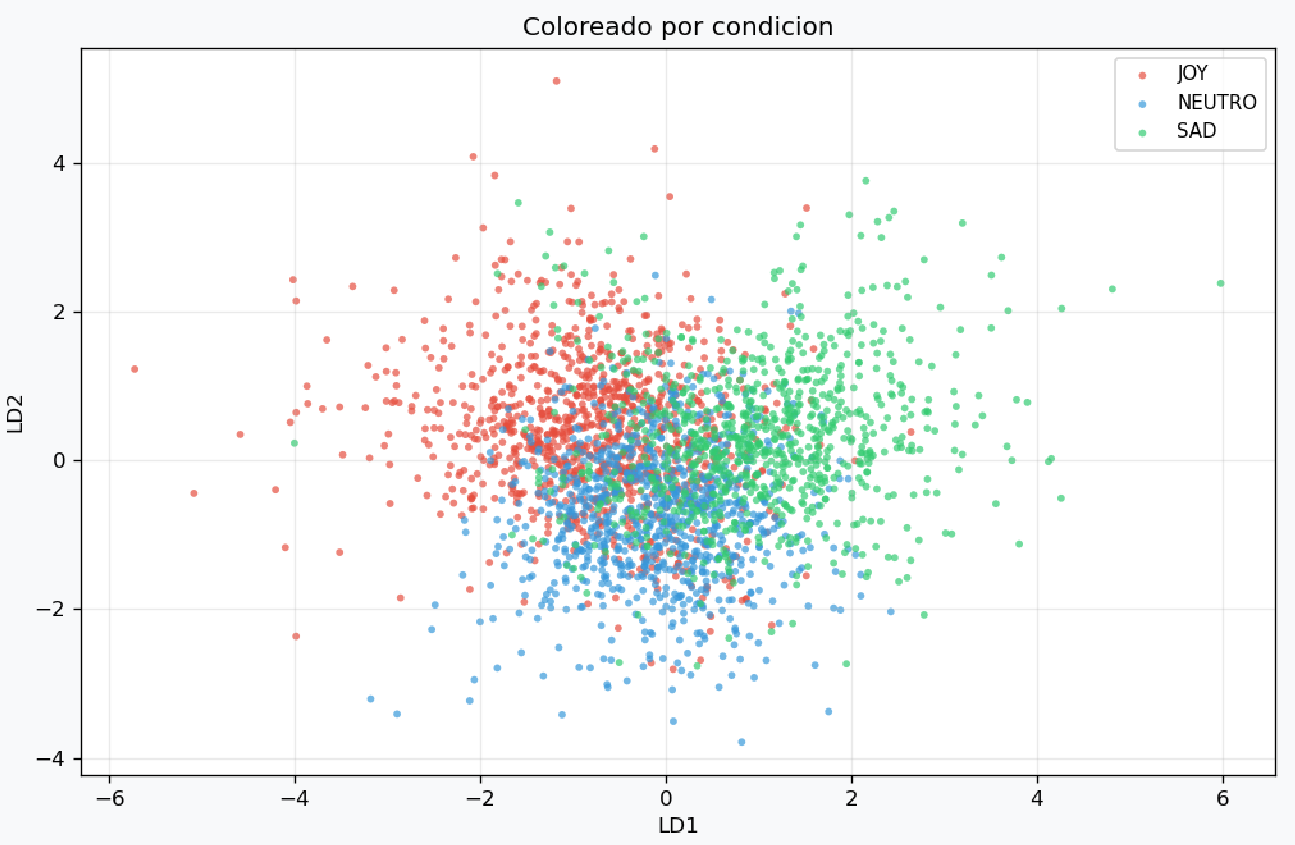
\includegraphics[width=0.94\linewidth]{../memoria/figs/separability/LDA_global_condicion.png}
            \vspace{1mm}

            {\scriptsize Color por condición emocional}
        \end{column}
        \begin{column}{0.49\textwidth}
            \centering
            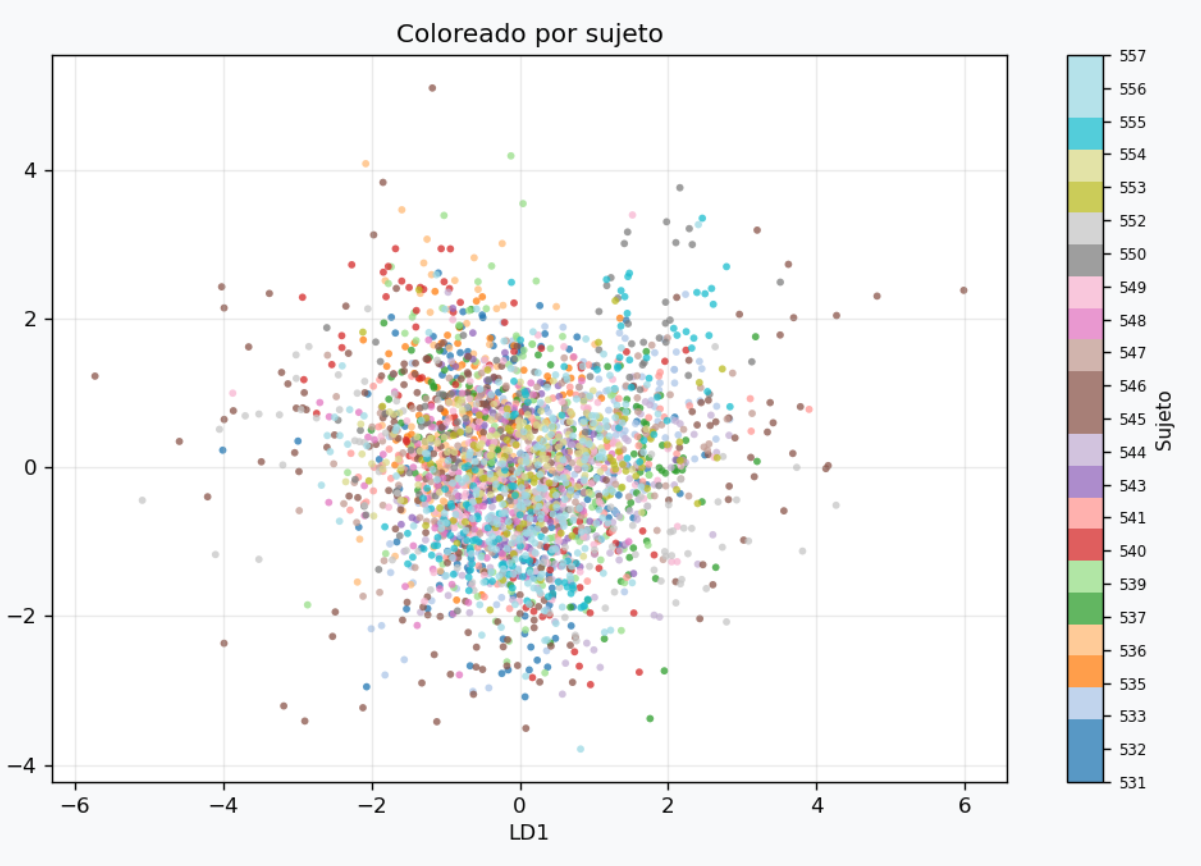
\includegraphics[width=0.94\linewidth]{../memoria/figs/separability/LDA_global_sujeto.png}
            \vspace{1mm}

            {\scriptsize Color por sujeto}
        \end{column}
    \end{columns}

    \vspace{3mm}
    \centering
    {\small La LDA busca una proyección más favorable para separar las emociones, pero sigue mostrando el efecto de la variabilidad entre sujetos.}
\end{frame}

\begin{frame}{Separabilidad por sujeto: PCA}
    \begin{columns}[T,onlytextwidth]
        \begin{column}{0.49\textwidth}
            \centering
            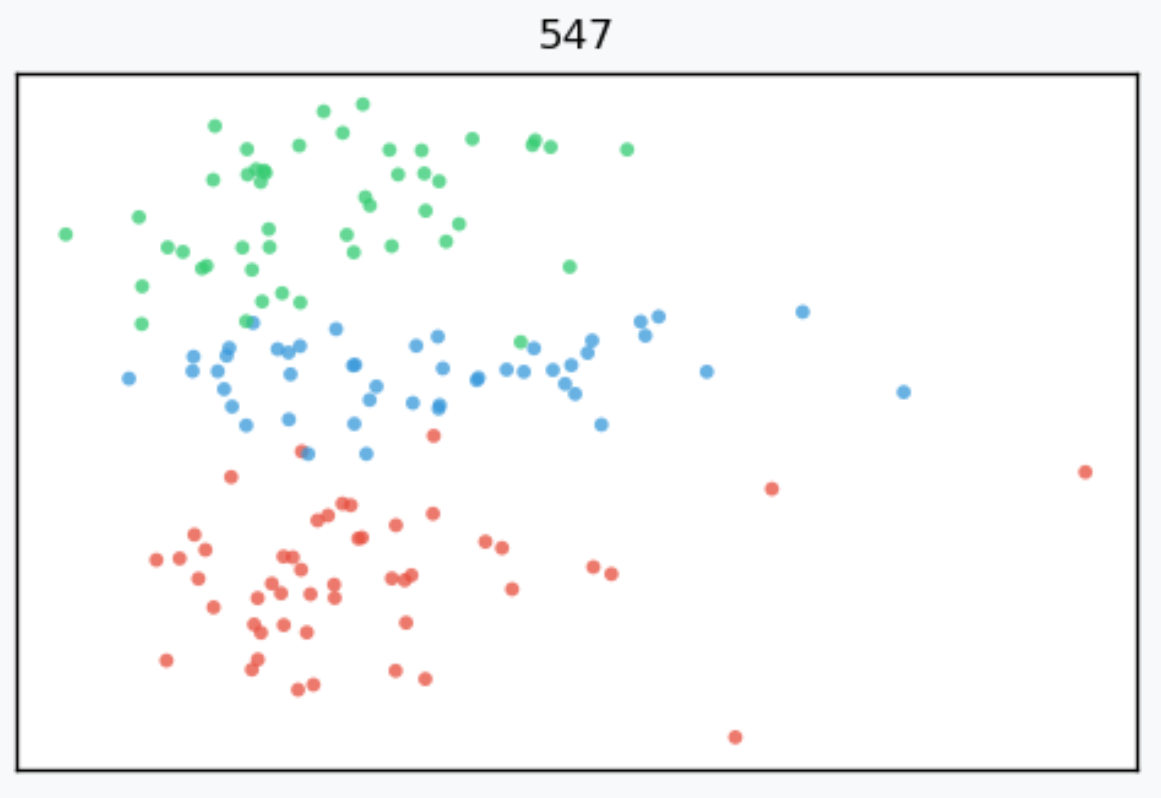
\includegraphics[width=0.88\linewidth]{../memoria/figs/separability/pca_547.png}
            \vspace{1mm}

            {\scriptsize Sujeto 211-000547}
        \end{column}
        \begin{column}{0.49\textwidth}
            \centering
            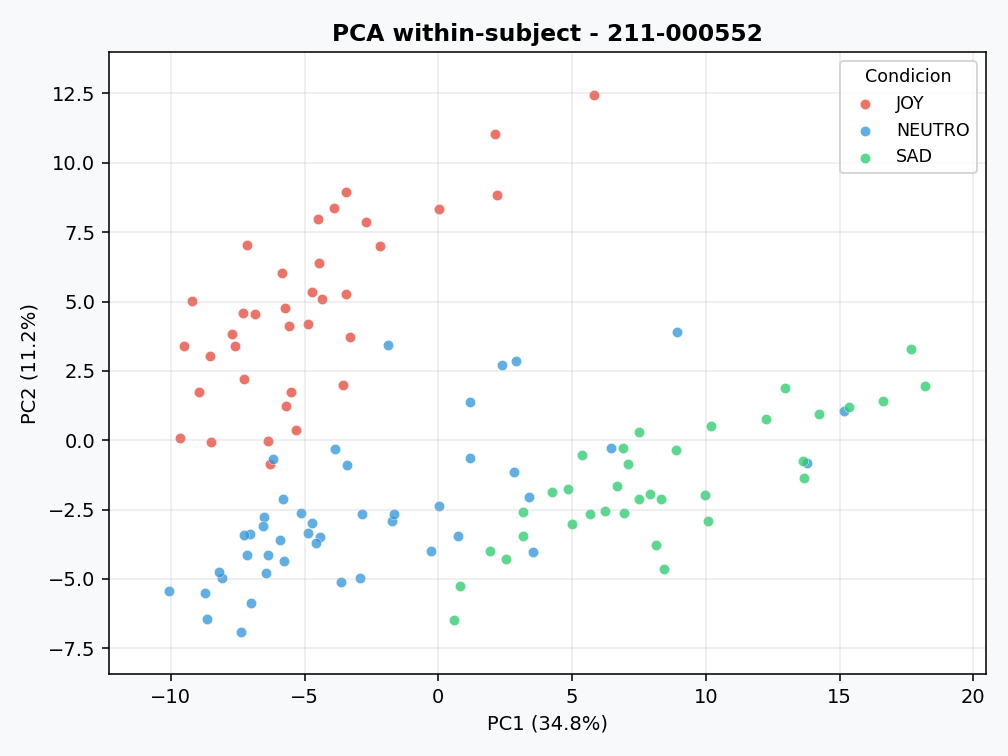
\includegraphics[width=0.88\linewidth]{../memoria/figs/separability/pca_552.png}
            \vspace{1mm}

            {\scriptsize Sujeto 211-000552}
        \end{column}
    \end{columns}

    \vspace{3mm}
    \centering
    {\small Al analizar cada participante por separado, la estructura emocional aparece menos mezclada que en el espacio global.}
\end{frame}

\begin{frame}{Separabilidad por sujeto: LDA}
    \begin{columns}[T,onlytextwidth]
        \begin{column}{0.49\textwidth}
            \centering
            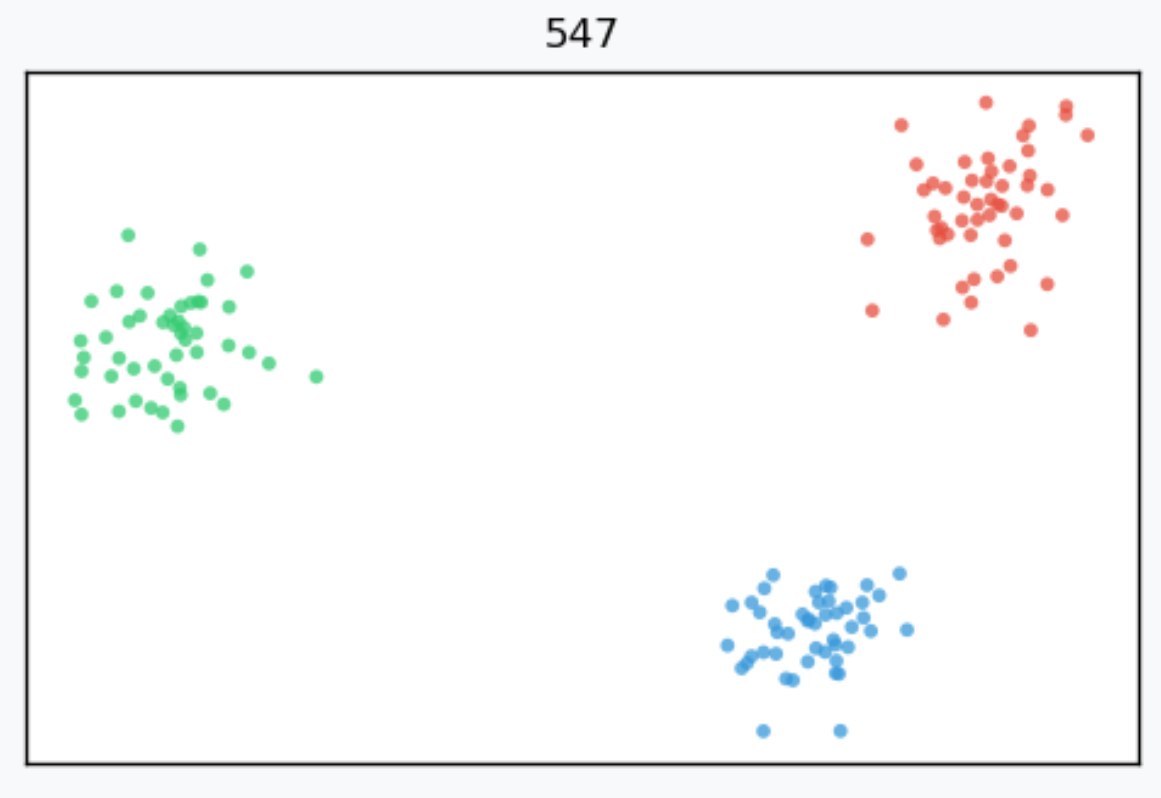
\includegraphics[width=0.88\linewidth]{../memoria/figs/separability/lda_547.png}
            \vspace{1mm}

            {\scriptsize Sujeto 211-000547}
        \end{column}
        \begin{column}{0.49\textwidth}
            \centering
            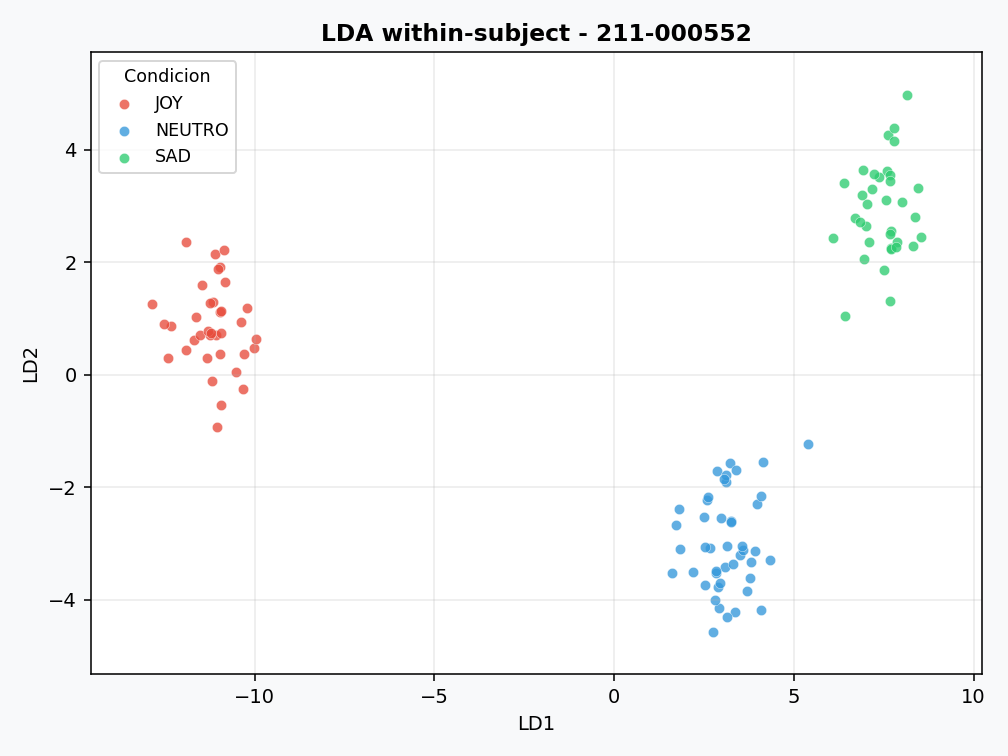
\includegraphics[width=0.88\linewidth]{../memoria/figs/separability/lda_552.png}
            \vspace{1mm}

            {\scriptsize Sujeto 211-000552}
        \end{column}
    \end{columns}

    \vspace{3mm}
    \centering
    {\small La separación dentro de cada sujeto es más clara, lo que anticipa un mejor comportamiento de los modelos personalizados.}
\end{frame}

\begin{frame}{Entrenamiento: regresión logística}
    \begin{columns}[T,onlytextwidth]
        \begin{column}{0.49\textwidth}
            \centering
            {\small\bfseries Modelo general}

            \vspace{1mm}
            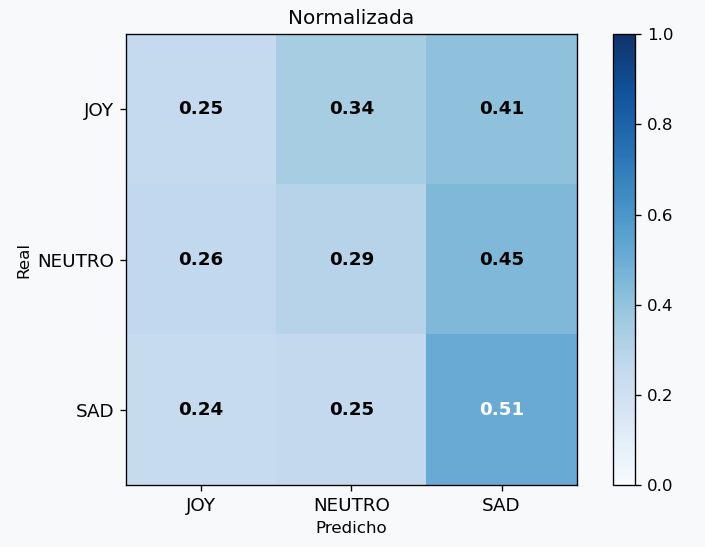
\includegraphics[width=0.92\linewidth]{../memoria/figs/training/all_subjects/log_reg.png}
        \end{column}
        \begin{column}{0.49\textwidth}
            \centering
            {\small\bfseries Modelo por sujeto}

            \vspace{1mm}
            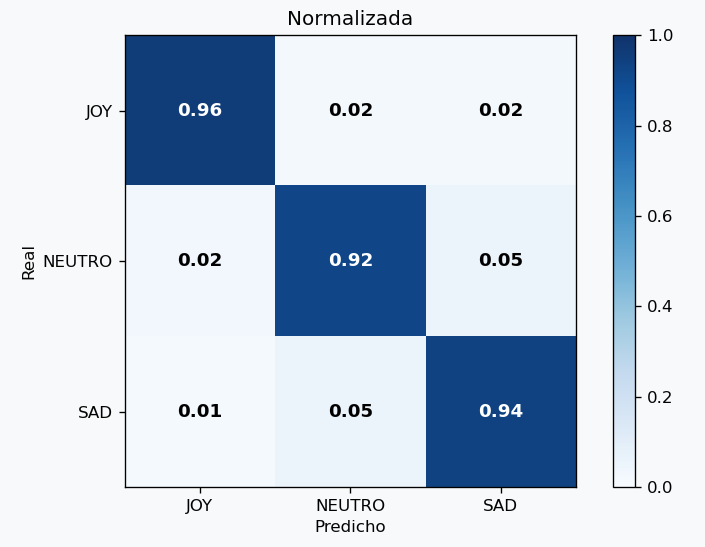
\includegraphics[width=0.92\linewidth]{../memoria/figs/training/within/logreg.png}
        \end{column}
    \end{columns}
\end{frame}

\begin{frame}{Explicabilidad: patrones emocionales}
    \begin{columns}[T,onlytextwidth]
        \begin{column}{0.31\textwidth}
            \begin{beamercolorbox}[rounded=true,sep=0.15cm,wd=\textwidth,center]{block body}
                {\bfseries JOY}\\[1.5mm]
                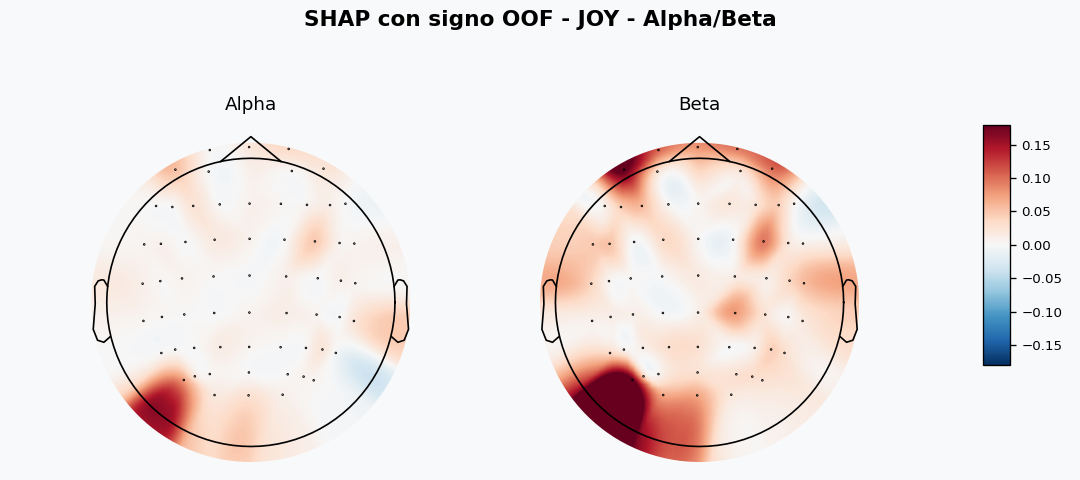
\includegraphics[width=0.90\textwidth]{../memoria/figs/explicabilidad/04_topomap_signed_JOY.png}

                \vspace{0.05cm}
                {\scriptsize frontal y posterior\\mayor implicación}
            \end{beamercolorbox}
        \end{column}

        \begin{column}{0.31\textwidth}
            \begin{beamercolorbox}[rounded=true,sep=0.15cm,wd=\textwidth,center]{block body}
                {\bfseries NEUTRO}\\[1.5mm]
                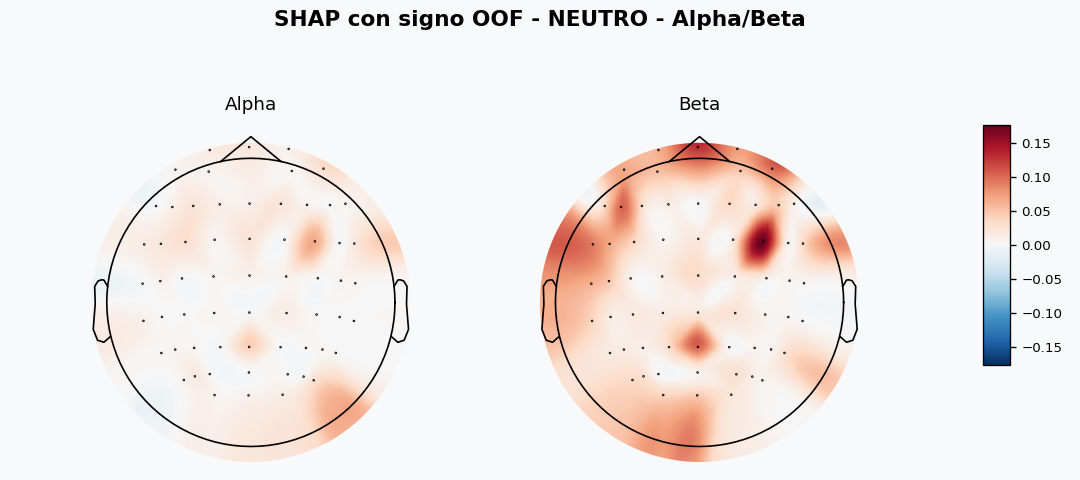
\includegraphics[width=0.90\textwidth]{../memoria/figs/explicabilidad/04_topomap_signed_NEUTRO.png}

                \vspace{0.05cm}
                {\scriptsize distribución más localizada\\referencia emocional}
            \end{beamercolorbox}
        \end{column}

        \begin{column}{0.31\textwidth}
            \begin{beamercolorbox}[rounded=true,sep=0.15cm,wd=\textwidth,center]{block body}
                {\bfseries SAD}\\[1.5mm]
                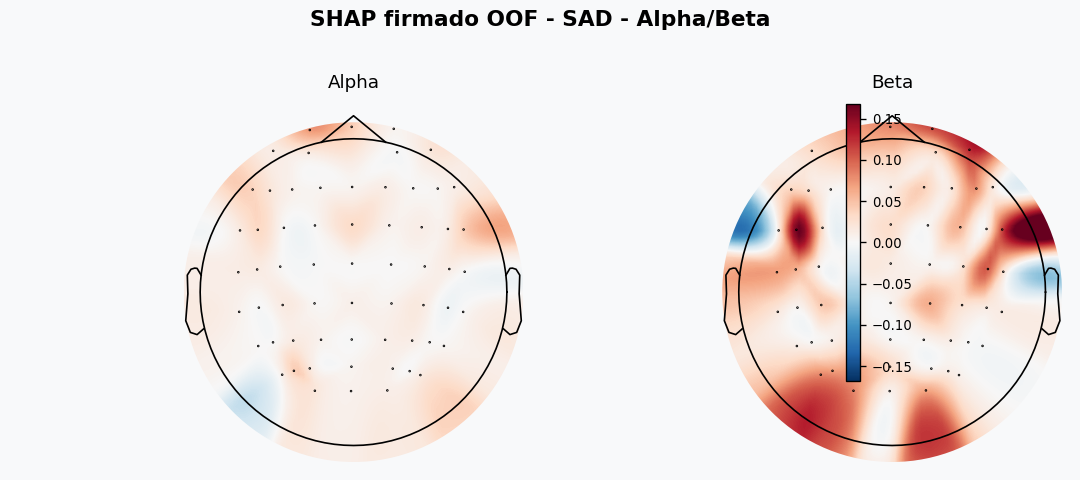
\includegraphics[width=0.90\textwidth]{../memoria/figs/explicabilidad/04_topomap_signed_SAD.png}

                \vspace{0.05cm}
                {\scriptsize temporal y posterior\\frontal menos homogéneo}
            \end{beamercolorbox}
        \end{column}
    \end{columns}

    \vspace{0.25cm}
    \begin{center}
        {\scriptsize Topomaps de importancia: muestran qué zonas y bandas usa el modelo para diferenciar clases.}
    \end{center}
\end{frame}
